\section{Scaling up Visual Model-Predictive Control}
\begin{figure*}
	\centering
	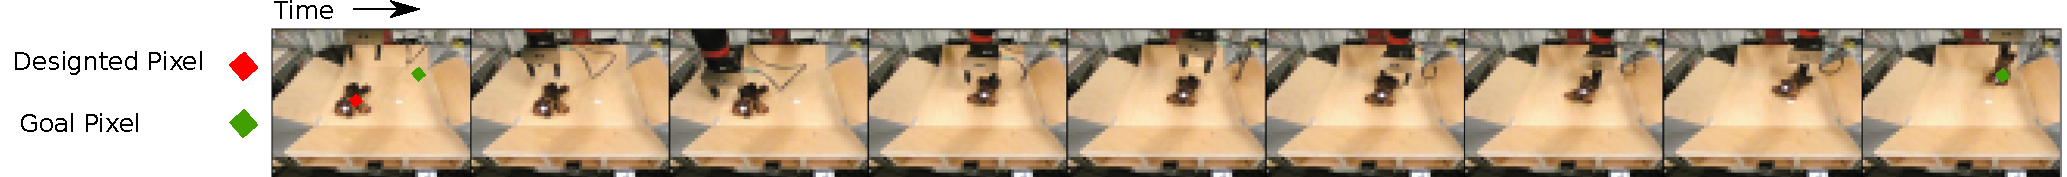
\includegraphics[width=1.0\textwidth]{images_rfr/pick_place_plush.pdf}
	\caption{\small{Retrying behavior of our method combining prehensile and non-prehensile manipulation. In the first 4 time instants shown the agent pushes the object. It then loses the object, and decides to grasp it pulling it all the way to the goal. Retrying is enabled by applying the learned registration to both camera views (here we only show the front view).}}
	\label{fig:push_grasp}
	
\end{figure*}

%%SL.10.15: Have transition here and explain what this section is about. Currently, it seems like a bunch of disjointed miscallaneous stuff that didn't fit in anywhere else. This is not good. Maybe you can call this system design and describe the robot setup here first (both single view and multi-view), then details about data collection -- how actions are selected etc. (which can be merged with 7.2). Figures would help to illustrate the robot setup. 7.3 probably doesn't belong here at all, but belongs in experiments

\label{sec:scalingup}
\subsection{Multi-view Visual MPC}
To allow disambiguating 3D-tasks, we extend visual MPC to include multiple camera views. Since tasks are defined in terms of pixel motion in 2D image space, the combination of multiple 2D tasks defines a 3D task, when cameras are oriented appropriately. In our experiments, we show that we can define 3D manipulation tasks, such as lifting an object from the table, that would be ambiguous using only a single camera view. The registration method described in the previous section is used separately per view to allow for dynamic retrying and solving temporally extended tasks. The planning costs from each view are combined using weighted averaging where the weights are provided by the registration network (see equation \ref{eqn:cost_avg}). 

\subsection{Learning complex Pick and Place Behavior with Visual MPC}
In prior work on video-prediction-based robotic manipulation \cite{sna, foresight}, the capabilities that emerged out of self-supervised learning were generally restricted to pushing and dragging objects. To enable more complex skills to emerge, we also explore how the sampling distribution used both for data collection and sampling-based planning can be changed to allow complex behavior such as picking and lifting objects for rearrangement as well as folding cloth can emerge. 

We first discuss picking and placing of objects. One of the main challenges with random exploration is that it is unlikely to pick up objects a sufficiently large fraction of the time to allow the model to learn grasping skills. To alleviate this issue, we incorporate a simple ``reflex'' during data collection, where the gripper automatically closes when the height of the wrist above the table is lower than a small threshold. This reflex is inspired by the palmar reflex observed in infants~\cite{grasping_fetal}. With this primitive, about 20\% of training trajectories included some sort of grasp on an object. It is worth noting that, other than this reflex, no grasping-specific engineering was applied to the policy allowing a joint pushing and grasping policy to emerge, see figure \ref{fig:push_grasp}. In our experiments, we evaluate our method using data obtained both with and without the grasping reflex, evaluating both purely non-prehensile and combined prehensile and non-prehensile manipulation.

\subsection{Learning Cloth-Folding with Visual-MPC}
 a major impediment is that when executing random actions clothes can become tangled pu

